% Source of DFD.pdf. Rebuild: pdflatex DFD.tex
\documentclass[tikz,border=2pt]{standalone}
\usepackage[T1]{fontenc}
\usepackage{helvet}
\renewcommand{\familydefault}{\sfdefault}
\usetikzlibrary{positioning,fit,arrows.meta,backgrounds,calc}
\begin{document}
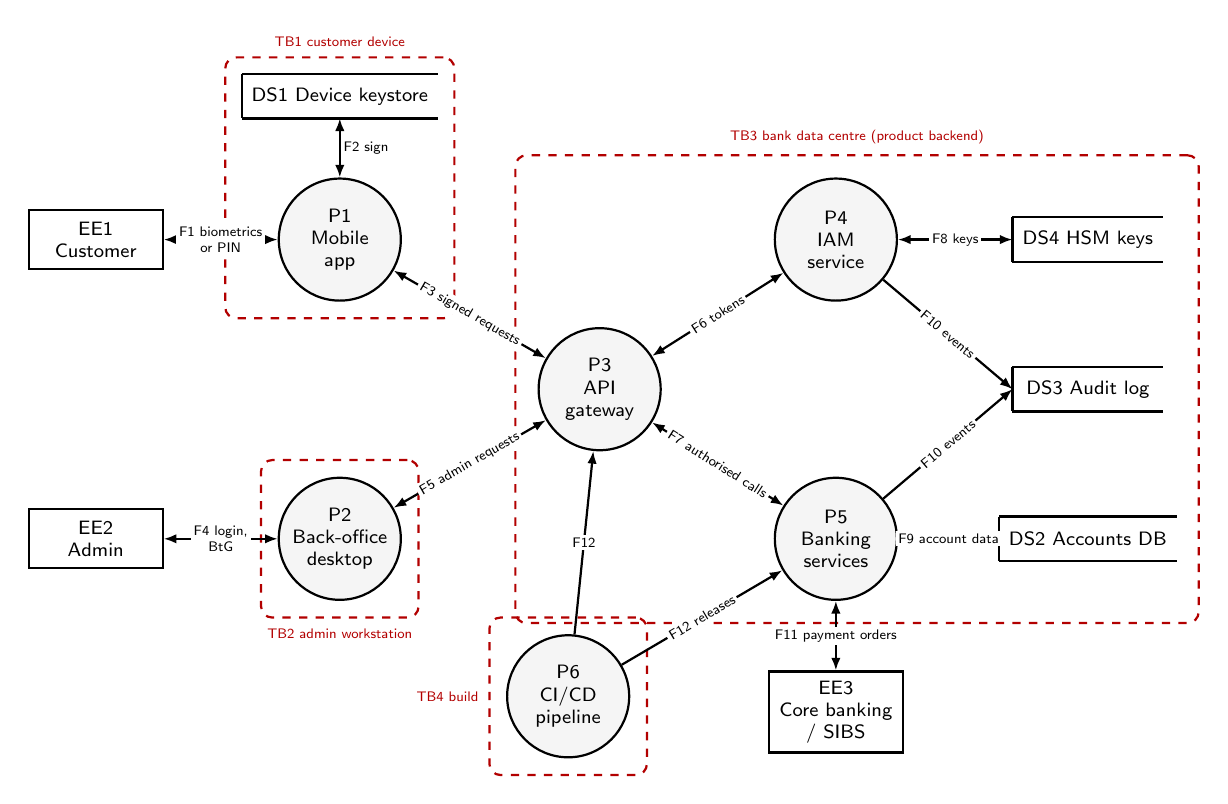
\begin{tikzpicture}[font=\scriptsize,
  ee/.style={draw,thick,minimum width=1.7cm,minimum height=0.75cm,align=center},
  proc/.style={draw,thick,circle,minimum size=1.55cm,align=center,inner sep=1pt,fill=gray!8},
  ds/.style={minimum width=1.9cm,minimum height=0.55cm,align=center,
    append after command={
      \pgfextra{\draw[thick] (\tikzlastnode.north west) -- (\tikzlastnode.north east)
                             (\tikzlastnode.south west) -- (\tikzlastnode.south east)
                             (\tikzlastnode.north west) -- (\tikzlastnode.south west);}}},
  arr/.style={-{Latex[length=1.6mm]},thick},
  barr/.style={{Latex[length=1.6mm]}-{Latex[length=1.6mm]},thick},
  lbl/.style={font=\tiny,fill=white,inner sep=1pt,align=center},
  tb/.style={draw,dashed,red!70!black,rounded corners,thick}]
% external entities
\node[ee] (cus) at (0,2.2) {EE1\\Customer};
\node[ee] (adm) at (0,-1.6) {EE2\\Admin};
% clients
\node[proc] (app) at (3.1,2.2) {P1\\Mobile\\app};
\node[ds,above=0.75cm of app] (key) {DS1 Device keystore};
\node[proc] (desk) at (3.1,-1.6) {P2\\Back-office\\desktop};
% backend
\node[proc] (gw) at (6.4,0.3) {P3\\API\\gateway};
\node[proc] (iam) at (9.4,2.2) {P4\\IAM\\service};
\node[proc] (svc) at (9.4,-1.6) {P5\\Banking\\services};
\node[ds] (hsm) at (12.6,2.2) {DS4 HSM keys};
\node[ds] (log) at (12.6,0.3) {DS3 Audit log};
\node[ds] (db) at (12.6,-1.6) {DS2 Accounts DB};
\node[proc] (ci) at (6.0,-3.6) {P6\\CI/CD\\pipeline};
\node[ee] (bank) at (9.4,-3.8) {EE3\\Core banking\\/ SIBS};
% flows
\draw[barr] (cus) -- node[lbl]{F1 biometrics\\or PIN} (app);
\draw[barr] (app) -- node[lbl,right]{F2 sign} (key);
\draw[barr] (app) -- node[lbl,sloped]{F3 signed requests} (gw);
\draw[barr] (adm) -- node[lbl]{F4 login,\\BtG} (desk);
\draw[barr] (desk) -- node[lbl,sloped]{F5 admin requests} (gw);
\draw[barr] (gw) -- node[lbl,sloped]{F6 tokens} (iam);
\draw[barr] (gw) -- node[lbl,sloped]{F7 authorised calls} (svc);
\draw[barr] (iam) -- node[lbl]{F8 keys} (hsm);
\draw[barr] (svc) -- node[lbl]{F9 account data} (db);
\draw[arr] (iam) -- node[lbl,sloped]{F10 events} (log.west);
\draw[arr] (svc) -- node[lbl,sloped]{F10 events} (log.west);
\draw[barr] (svc) -- node[lbl]{F11 payment orders} (bank);
\draw[arr] (ci) -- node[lbl,sloped]{F12 releases} (svc);
\draw[arr] (ci) -- node[lbl]{F12} (gw);
% trust boundaries
\begin{scope}[on background layer]
\node[tb,fit=(key)(app),inner sep=6pt,label={[red!70!black,font=\tiny]above:TB1 customer device}] {};
\node[tb,fit=(desk),inner sep=6pt,label={[red!70!black,font=\tiny]below:TB2 admin workstation}] {};
\node[tb,fit=(ci),inner sep=6pt,label={[red!70!black,font=\tiny]left:TB4 build}] {};
\node[tb,fit=(gw)(iam)(svc)(hsm)(log)(db),inner sep=8pt,label={[red!70!black,font=\tiny]above:TB3 bank data centre (product backend)}] {};
\end{scope}
\end{tikzpicture}
\end{document}
